\chapter{Evaluation strukturierter p2p Overlay-Netzwerke}
\label{chap:evaluation_p2p}

Dieses Kapitel bietet einen Überblick über einige p2p-Netzwerke und evaluiert diese anhand gestellter Anforderungen. Diese Evaluation beeinflusst die Entscheidung für ein Overlay-Netzwerk, das die Grundlage des zu entwickelnden verteilte Publish/Subscribe-System bildet. Diese Evaluation bedient sich zahlreicher Arbeiten, die sich alleine dem Vergleich dieser Netzwerke widmen \cite{Lua2005Survey, Goetz2005, Li2004Comparing, Darlagiannis2006Peertopeer, Castro2002Secure, Bo2003PeertoPeer} und geht auch auf ihre Nutzbarkeit als Basis für \emph{Application level multicast} sprich ein Publish/Subscribe-System ein \cite{Hosseini2007Survey, Fahmy2007, Castro2003Evaluation, Ratnasamy2001}.

Zuvor müssen jedoch die Anforderungen von \acp{mmve} an solche Systeme identifiziert werden. Diese Anforderungen werden bei der Auswahl der Netzwerkes in Betracht gezogen.

\section{Anforderungen an p2p-Netzwerke}

\paragraph{Geringe Latenz} Schnelle Reaktionszeiten und Nachrichtenübermittlung sind bei \ac{mmog} unverzichtbar. Ebenfalls müssen größere Nachrichten schnell übertragen werden, damit der Informationsfluss zur korrekten Darstellung der virtuellen Umgebung nicht behindert wird. Dies lässt sich beispielsweise anhand der Anzahl der Hops beim Nachrichtenversand messen, ist aber letzlich abhängig von der zur Verfügung stehenden Bandbreite jedes einzelnen Knotens.

\paragraph{Skalierbarkeit und Fehlertoleranz bei Knotenausfall} Selbst bei einer großen Anzahl an Knoten soll das Netz nicht kollabieren. Hierbei ist es auch wichtig, dass Knoten keine erforderliche Durchschnittszeit im Netz integriert sein müssen. Es kann davon ausgegangen sein, dass ein durchschnittlicher Spieler eines \acp{mmog} längere Zeit im Spiel angemeldet ist. Li untersucht in \cite{Li2004Comparing} wie sich p2p-Netzwerke bei großen Fluktuationen verhalten.

\paragraph{Kommunikation über das Netzwerk} Das Netzwerk soll nicht nur das schnelle Auffinden von Peers ermöglichen, sondern auch einen Transport der Nachricht (Routing) durch das Netzwerk selbst bereitstellen.

\paragraph{Eingriff in Routingentscheidungen} Applikationswissen hilft auch beim Eingriff in das Routing des Netzes. So können Knoten bevorzugt zur Weiterleitung einer Nachricht ausgewählt werden. Diese Knoten zeichnen sich beispielsweise durch eine große Bandbreite oder spezielle Applikationsmetriken\footnote{Bsp: Spieler befindet sich in der selben Stadt} aus.

\paragraph{Verfügbarkeit als C/C++-Bibliothek} Da der Prototyp dieser Arbeit in C++ entwickelt wird, muss das Netzwerk als C/C++-Bibliothek verfügbar sein. So kann das Netzwerk einfach angesprochen werden ohne dass kostenintensive Brücken zwischen beispielsweise Java und C++ geschlagen werden müssen. Da zudem betriebssystemübergreifend entwickelt und getestet wird, ist außerdem ein zur Verfügung stehender Quellcode vorteilhaft.

\paragraph{Anpassbarkeit an generische KBR-API}
Das gewählte System sollte mit der von Dabek beschriebenen generische KBR-API\footnote{siehe \Fref{chap:grundlagen:api}} kompatibel sein.

\section[Evaluation dreier p2p-Netzwerke]{Evaluation der der Netzwerke Chord, Pastry/Tapestry und CAN}
In diesem Kapitel werden die vier bekannten Systeme Chord \cite{Stoica2003}, Pastry \cite{Rowstron2001}, Tapestry \cite{Zhao2001Tapestry,Zhao2004Tapestry} und CAN \cite{Ratnasamy2001Scalable} miteinander verglichen. Die ersten drei sind in ihrem Aufbau ähnlich (der Schlüsselraum ist auf einem Ring verteilt) und unterscheiden sich in der Art des Routings. CAN hingegen bildet den Schlüsselraum auf ein d-dimensionales kartesisches Koordinatensystem ab. Alle vier Systeme sind laut \cite{Dabek2003Towards} an die generische \ac{api} anpassbar.

\subsection{Chord}
\label{chap:evaluation_chord}

\subsubsection{Aufbau und Struktur}
Chord \cite{Stoica2003} legt die $l$ bit wertigen Schlüssel (meist Zahlen im Bereich $[0,2^l-1]$) auf einem eindimensionalen Ring modulo $2^l$ im Uhrzeigersinn an. Jedem Knoten und jedem Datensatz ist ein eindeutiger Schlüssel zugewiesen, diese werden \emph{ID} und \emph{key} genannt. Ein Datensatz $X$ ist dem Knoten zugewiesen, dessen ID größer gleich dem key ist. Dieser Knoten wird Nachfolger von X, \emph{SUCC(X)}, genannt. Analog dazu gibt es auch einen Vorgänger von X, \emph{PRED(X)}.

\begin{figure}[htbp]
\centering
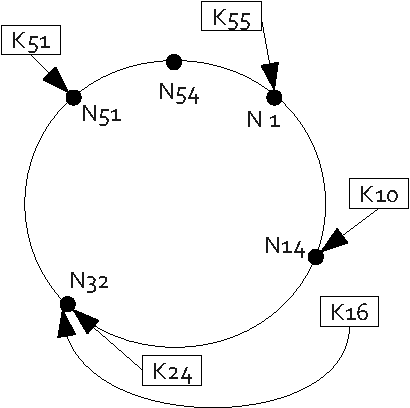
\includegraphics{grafics/chord_key_space.pdf}
\caption{Schlüsselraum für Chord mit sechs Knoten ($Nx$) und fünf Daten ($Kx$)}
\label{fig:chord_key_space}
\end{figure}

Damit ist ein Knoten für alle Daten zuständig, die -- bildlich gesehen -- im Ring gegen den Uhrzeigersinn vor ihm liegen. In \Fref{fig:chord_key_space} ist dies mit $l=6$ für sechs Knoten und fünf Datenpunkten gezeigt. Knoten 14 (N14) ist für den Datensatz mit Schlüssel 10 (K10) zuständig. Knoten 32 ist für K16 und K24 verantwortlich. K51 ist bei N51 zu finden. Aufgrund der Ringstruktur ist N1 für K55 zuständig. Die gestrichelten Pfeile stellen die Einträge der sogenannten Fingertabelle für Knoten $N1$ dar. 

\subsubsection{Routing}
Bei Chord besitzt jeder Knoten eine Verbindung zu seinem direkten Vorgänger und seinem direkten Nachfolger. Eine Nachricht wird von jedem Knoten so lange an seinen Nachfolger geschickt, bis sie zum zuständigen Knoten gelangt. Bei einer \texttt{lookup(x)}-Nachricht\footnote{Suche für key x Knoten N, so dass gilt: $N = SUCC(x)$.} prüft jeder involvierte Knoten A, ob sein Nachfolger für den Schlüssel zuständig ist, d.h. $ID_A < x \le SUCC(A)$. Ist dies der Fall, so sendet Knoten A die Antwort $SUCC(A)$ zurück. Bei normalem Nachrichtenaustausch wird die Nachricht zur Behandlung an den zuständigen Knoten weitergeleitet.

Da dies eine sehr ineffizientes  Routing darstellt, pflegt jeder Knoten eine Fingertabelle. Die maximal $l$ Einträge in dieser Tabelle zeigen auf andere Knoten im Ring, so dass der Eintrag in Zeile $i$ von Knoten $n$ denjenigen Knoten enthält, dessen ID mindestens um $2^{i-1}$ größer ist als $ID_n$.\\
In \Fref{fig:chord_key_space} ist die Fingertabelle von Knoten $N1$ mit ID$_{N1} = 1$ dargestellt. Die Einträge berechnen sich wie folgt: In der ersten Zeile (Idx 0) steht der Knoten, dessen ID um $2^{1-1} = 1$ größer ist, als die ID$_{N1}$. Dies ist $SUCC(2)$ und zeigt auf Knoten $N5$. In der dritten Zeile (Idx 2) findet sich der Knoten dessen ID mindestens um $2^{3-1} = 4$ größer ist als ID$_{N1}$, also $SUCC(5)$ und damit ebenfalls auf Knoten $N5$. Der vierte Eintrag verweist demnach auf $SUCC(9) = N14$. Analog dazu berechnen sich die restlichen Einträge.

Über diese Fingertabelle können Nachrichten eine größere Strecke auf dem Ring überbrücken und die Routingzeit wird stark verkürzt. Da die IDs in der Tabelle exponentiell zur Basis $2$ ansteigen, halbiert sich die Distanz zum Ziel. Damit besitzt das Routing eine Komplexität von $O(log N)$.

\subsubsection{Nachbarschaft}
Die Nachbarschaft ist bei Chord begrenzt. Jeder Knoten hat eine Verbindung zu seinem Vorgänger sowie Nachfolger auf dem Ring und hält Einträge in der Fingertabelle vor. In die Routingentscheidungen kann nicht direkt eingegriffen werden.

\subsubsection{Eintritt und Austritt (Fehlerfall) von Knoten}
Bei Chord kann die ID für einen neuen Knoten $n$ frei aus dem Wertebereich des Schlüsselraums gewählt werden, es muss lediglich ein Knoten $b$ im System bekannt sein. $n$ routet eine \texttt{lookup(n)}-Nachricht via $b$ und erfährt somit, wer sein Nachfolger auf dem Ring ist. In gleicher Weise vervollständigt $n$ seine Fingertabelle. Weiterhin teilt $n$ seinem Nachfolger mit, dass $n$ nun sein neuer Vorgänger ist.

Zur Stabilisierung und Vervollständigung der Routinginformationen arbeitet jeder Knoten im Ring periodisch die Funktion \texttt{stabilize} ab. Jeder Knoten $a$ fragt seinen Nachfolger $n$ nach dessen Vorgänger $s$. Wenn $s$ ungleich $a$ ist, muss Knoten $s$ neu in den Ring eingetreten sein. $a$ informiert den neuen Knoten $s$, dass er sein Vorgänger ist und ändert selbst den eigenen Nachfolger auf $s$ ab. $s$ kennt nun den Bereich seiner Zuständigkeit $[ID_a, ID_s[$, fordert diese Daten von seinem Nachfolger an und weist diesen auf die Zuständigkeitsänderung hin.\\
Die Aktualisierung der Fingertabelle \texttt{fix\_fingers} wird ebenfalls auf jedem Knoten periodisch angestoßen. Für einen zufällig gewählten Eintrag wird überprüft, ob dieser noch aktuell ist.

Die verzögerte Aktualisierung hat keinen großen Einfluss auf die Korrektheit oder Geschwindigkeit des Routings, da eine fehlerhafte Nachrichtenzustellung über die Nachfolger- beziehungsweise Vorgängerverbindungen des empfangenden Knotens weitergeleitet wird.

\begin{figure}[htbp]
\centering
\resizebox{\textwidth}{!}{%
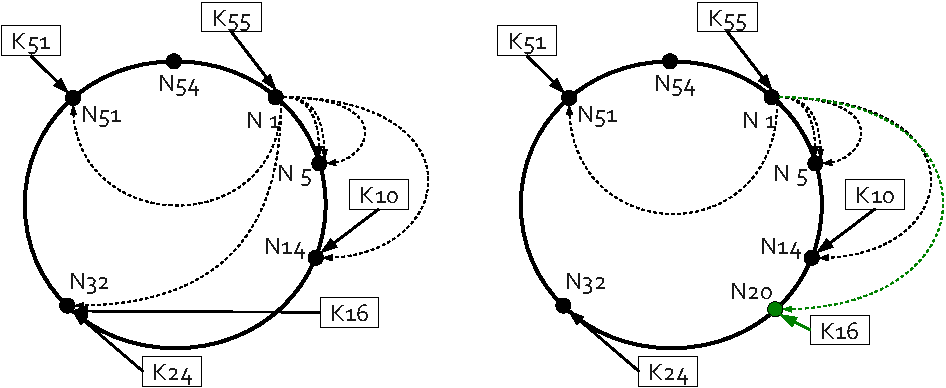
\includegraphics{grafics/chord_new_node.pdf}}
\caption{Schlüsselraum von Chord nach Ankunft von Knoten $N20$}
\label{fig:chord_new_node}
\end{figure}

\Fref[plain]{fig:chord_new_node} verdeutlicht den Neueintritt von Knoten $N20$. Die Änderungen sind in Grün dargestellt: $N1$ passt seine Fingertabelle an und $N20$ ist für $K16$ zuständig.

Der Ausfall von Knoten wird über \emph{Timeouts} ermittelt. Im Falle eines Timeouts wird die Nachricht an den besten bekannten Vorgänger des ausgefallenen Knotens weitergeleitet. Im schlimmsten Falle ist dies der Nachfolger des sendenden Knotens. Daraus wird ersichtlich, dass ein valider Nachfolger notwendig ist. Aus diesem Grund hält jeder Knoten eine Liste von möglichen Nachfolgern vor, die während \texttt{stabilize} erstellt werden. Für fehlerhafte Knoten in der Fingertabelle kann \texttt{fix\_fingers} explizit aufgerufen werden.
Knotenausfall bedeutet nicht nur einen Ausfall des Knotens, sondern bedingt, dass die dort gespeicherten Daten nicht mehr erreichbar sind.\\
Verlässt ein Knoten das Netz, so beeinflusst dies das System nicht. Jedoch ist es effizienter, wenn ein verlassender Knoten seinem Vorgänger und Nachfolger dies mitteilt, die Verbindungen angepasst werden und die Datensätze explizit übertragen werden.

\subsection{Pastry/Tapestry}
\label{chap:evaluation_pastry}

\subsubsection{Aufbau und Struktur}
Pastry \cite{Rowstron2001} und Tapestry \cite{Zhao2001Tapestry,Zhao2004Tapestry} sind sich sehr ähnlich, da beide auf Plaxtons Arbeit \cite{Plaxton1997Accessing} aufbauen. Daher wird auf Tapestry nicht näher eingegangen, da die Unterschiede für das Konzept dieser Systeme nicht relevant sind.

Pastry besitzt wie Chord einen $l$ bit-wertigen Schlüsselraum, dabei werden Schlüssel als Zahlen zur Basis $2^b$ dargestellt, wobei die Wahl von $b$ einen Einfluss auf das Routing hat, da dieser die Größe der Routingtabelle beeinflusst. Ein Datensatz ist dem Knoten zugewiesen, dessen ID den kleinsten Abstand zum Schlüsselwert des Datensatzes hat.\\
\Fref{fig:pastry_key_space} zeigt dies beispielhaft für die gleichen sechs Knoten und fünf Datensätze wie in \Fref[plain]{fig:chord_key_space}. Im Unterschied zu Chord ist jedoch Knoten $N14$ für $K16$ und Knoten $N54$ für $K55$ zuständig.


\begin{figure}[htbp]
\centering
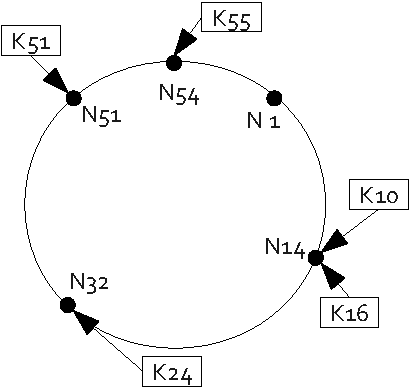
\includegraphics{grafics/pastry_key_space.pdf}
\caption{Schlüsselraum für Pastry mit sechs Knoten ($Nx$) und fünf Daten ($Kx$)}
\label{fig:pastry_key_space}
\end{figure}

\subsubsection{Routing}
Jeder Knoten verwaltet neben den ihm zugeteilten Datensätzen drei Strukturen, die dem Routing dienen. Diese sind das \emph{leaf set} mit Einträgen zu Knoten, die im Schlüsselraum benachbart sind, das \emph{neighborhood set} mit Einträgen zu Knoten, die aus Netzwerksicht nahe liegen, und die Routingtabelle selbst. In \Fref{fig:pastry_routing_table} sind nur die Schlüssel, nicht aber Kontaktinformation, wie IP-Adresse und Port dargestellt.

\begin{figure}[htbp]
\centering
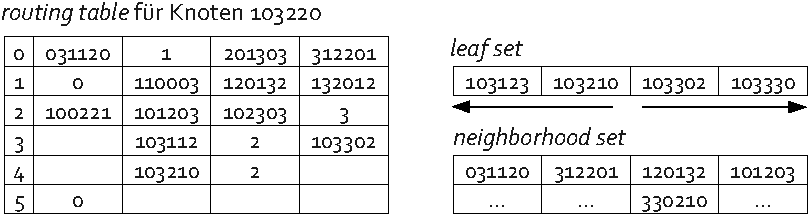
\includegraphics{grafics/pastry_routing_table.pdf}
\caption{Routing table, leaf set und neighborhood set bei Pastry}
\label{fig:pastry_routing_table}
\end{figure}

Die Routingtabelle besteht aus $\frac{l}{b}$ Reihen mit je $2^b -1$ Einträgen. \Fref{fig:pastry_routing_table} zeigt dies beispielhaft für Knoten $103220$ mit $l=12, b=2$ (nach \cite{Goetz2005}). Einträge in Zeile $i$ haben einen Präfix der Länge $i$ mit dem Knoten $103220$ gemein. Die Übereinstimmungen sind in der Abbildung fett hervorgehoben. Ist kein passender Knoten bekannt, wird das entsprechende Feld nicht ausgefüllt. Damit hat die Routingtabelle Ähnlichkeiten zur Fingertabelle bei Chord. Ein Knoten hat ungenaues Wissen über entfernte Knoten. Der Detailgrad an Routinginformationen erhöht sich pro Zeile in der Routingtabelle. Sind im System wenig Knoten vorhanden, sind die letzten Reihen der Routingtabelle spärlich belegt. Im Durchschnitt sind bei $n$ Knoten im System nur $log_{2^b} n$ Einträge ausgefüllt.\\
Bei der Belegung der Routingtabelle werden bei gleichem Präfix diejenigen Knoten gewählt, die aus Netzwerksicht näher sind.

Das leaf set enthält die $l$ numerisch nahen Knoten, $\frac{l}{2}$ davon sind kleiner und $\frac{l}{2}$ größer als der aktuelle Knoten. Neben Informationen zu Routingentscheidungen wird es zur Reparatur genutzt, sollten nahe gelegene Knoten ausfallen.

Das eigentliche Routing unterscheidet zwei Fälle: Zuerst prüft der Knoten, ob der Schlüssel $k$ im Bereich seines leaf sets ist. Ist dies der Fall, wird die Nachricht an den entsprechenden Knoten gesendet. Ist dieser Knoten für den Schlüssel zuständig, endet das Routing. Fällt $k$ nicht in den Bereich des leaf sets, wird die Nachricht via Routingtabelle an einen weiter entfernten Knoten gesendet. Hierzu wird ein Eintrag gewählt, der eine größere beziehungsweise die größte Präfixübereinstimmung mit $k$ hat. Existiert kein solcher Eintrag, wird die Nachricht an den numerisch nächsten Knoten (zu $k$) mit gleicher Präfixübereinstimmung geschickt.\\
Da Nachrichten immer an Knoten mit einer größeren Übereinstimmung oder an nähere Knoten mit gleicher Präfixübereinstimmung gesendet werden, können keine Zyklen auftreten.

Dadurch verringert sich die Anzahl der Knoten mit längeren Präfixübereinstimmungen in jedem Schritt um mindestens den Faktor $2^b$. Somit hat das Routing eine Komplexität von $O(log_{2^b} N)$.

\subsubsection{Nachbarschaft}
Das neighborhood set (siehe \Fref[plain]{fig:pastry_routing_table}) enthält $|m|$ Knoten, die aus Netzwerksicht nahe sind. Obwohl es im Routing keine Rolle spielt, kann es dazu genutzt werden, um geeignete Knoten zu finden. Da die Größe des leaf sets ebenfalls wählbar ist, können hier auch vermehrt nahe Knoten platziert werden.

\subsubsection{Eintritt und Austritt (Fehlerfall) von Knoten}
Einem neuen Knoten $n$ wird von Applikationsseite ein frei wählbarer Schlüssel gegeben. Meist berechnet sich dieser Schlüssel anhand des Hashwerts über die IP oder seines öffentlichen Namens. Weiterhin geht das System davon aus, dass $n$ aus einer Liste bekannter Knoten denjenigen Knoten $x$ wählen kann, der aus Netzwerksicht nahe ist. Von diesem Knoten kann das neighborhood set kopiert werden. Zum Aufbau der Routingtabelle und des leaf sets lässt $n$ via $x$ eine \texttt{JOIN}-Nachricht an einen numerisch nahen Schlüssel zu $n$ routen. Diese Nachricht gelangt schließlich zu Knoten $c$, von dem das leaf set (die Liste der $l$ numerisch nahen Knoten) kopiert werden kann. Alle Knoten, die diese \texttt{JOIN}-Nachricht weiterleiten, senden ihre Routingtabelle an $n$. Für jeden Routinghop kopiert sich $n$ die entsprechende Zeile aus der Routingtabelle, da ausgehend von keiner Präfixübereinstimmung mit dem nahen Knoten $x$, jeder weitere Hop eine größere Präfixübereinstimmung bringt.\\
Im Gegensatz zur nachträglichen Aktualisierung bei Chord wird hier die gesamte Routinginformation an alle bekannten Knoten gesendet. Der neue Knoten ist nun im Netzwerk bekannt und erreichbar.

Ausgefallene Knoten werden ebenfalls anhand von Timeouts beim Routing entdeckt. Da die Einträge des neighborhood sets nicht im Routing involviert sind, müssen diese periodisch geprüft werden. Fehlerhafte Einträge in der Routingtabelle können über einen anderen Eintrag mit gleicher Präfixübereinstimmung kompensiert werden, müssen aber entfernt werden, um ein stabiles und sicheres Routing zu gewährleisten. Hierzu können von benachbarten Einträgen Routinginformationen angefordert werden, um die entstandene Lücke zu füllen. Ein fehlerhafter Eintrag im leaf set oder neighborhood set kann auf ähnliche Weise repariert werden: Hier werden Informationen von anderen, im leaf set oder neighborhood set eingetragenenen, Knoten angefordert.

Der Austritt eines Knotens wird vom System wie ein Fehlerfall behandelt. Um die Datenintegrität zu gewährleisten und um unnötigen Nachrichtenversand im System zu vermeiden, sollte die Applikation den Austritt eines Knotens jedoch speziell behandeln.


\subsection{CAN}
\label{chap:evaluation_can}

\subsubsection{Aufbau und Struktur}
Der Schlüsselraum bei CAN \cite{Ratnasamy2001Scalable} ist ein d-dimensionaler Torus. Die Schlüssel werden als d-Tupel (zum Beispiel $(x,y)$ für $d=2$) dargestellt. Wie bei Pastry ist der numerisch nächst gelegene Knoten für einen Datensatz zuständig. Der Schlüsselraum ist in nicht überlappende Zonen eingeteilt und hat eine feste Größe. Jeder Knoten \emph{besitzt} eine solche Zone, über deren Ausmaß er definiert ist. Er ist für alle Daten zuständig, deren Schlüssel in dieser Zone liegt. Ein Schlüssel wird, wie bei \ac{dht} üblich, über eine segmentierte Hashfunktion berechnet\footnote{Siehe \Fref{chap:dht} im Anhang}. Jedes Segment bildet dabei eine Dimension ab.

\Fref{fig:can_key_space} zeigt einen zweidimensionalen Schlüsselraum mit den drei Knoten A, B und C und fünf Datesätzenn, die als schwarze Punkte dargestellt sind. Der Schlüsselraum ist komplett auf die drei Knoten aufgeteilt, wobei A für den Bereich $(0, .5)-(1, 1)$, B für $(0, 0)-(.5, .5)$ und C für $(.5, 0)-(1, .5)$ zuständig ist.

\begin{figure}[htbp]
\centering
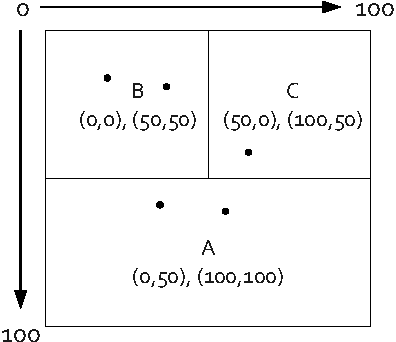
\includegraphics{grafics/can_key_space.pdf}
\caption{Zweidimensionaler Schlüsselraum für CAN}
\label{fig:can_key_space}
\end{figure}

\subsubsection{Routing} 
Die gespeicherte Routinginformation ist bei CAN am geringsten: Jeder Knoten speichert lediglich seine Nachbarn, das sind Knoten deren Zonen angrenzend sind, ab. Über die Zoneninformation jedes Nachbarn wird nun das Routing bestimmt. Eine Nachricht wird über den Knoten geschickt, der aufgrund seiner Zoneninformation dem Ziel am nächsten ist.

In \Fref{fig:can_routing} hat Knoten N1 die vier Knoten N2, N3, N4 und N5 als Nachbarn. Knoten N4 hingegen ist nur mit N1 und N5 benachbart. Eine Nachricht von $N1$ zu $K$ wird beispielsweise via Knoten $N5$ geroutet. Eine alternative Route via $N2$ ist gestrichelt dargestellt.

\begin{figure}[htbp]
\centering
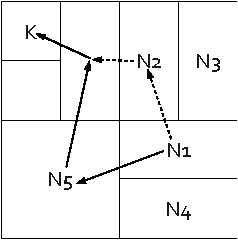
\includegraphics{grafics/can_routing.pdf}
\caption{Routing und Nachbarschaft bei CAN}
\label{fig:can_routing}
\end{figure}

Die durchschnittliche Länge eines Pfades bei $d$ Dimensionen und $n$ Knoten ist $O(d\cdot n^\frac{1}{d})$. Sind die Zonen gleich aufgeteilt, so besitzt jeder Knoten max. $2d$ Nachbarn und die Anzahl an Hops verringert sich auf $O(\frac{4}{d}\cdot n^\frac{1}{d})$.

\subsubsection{Nachbarschaft}
Die Nachbarschaft von CAN wurde bereits im vorigen Abschnitt behandelt. Dank deren Einfachheit ist der Ein- und Austritt von Knoten zwar besonders einfach und tangiert nur wenige Knoten im Netz, jedoch kann auf die Nähe aus Netzwerksicht nur beim Eintritt eines Knotens bei der Wahl seiner Koordinaten Rücksicht genommen werden.

Die Erhöhung der Dimension bedingt eine größere Nachbarschaft und damit, neben einem kürzeren Routing, auch die Möglichkeit, mehr Knoten in der Nachbarschaft anzusiedeln. Zusätzlich können in CAN sogenannte \emph{Realitäten} genutzt werden. Dies sind verschiedene CAN-Netzwerke mit unterschiedlichen Hashfunktionen zur Berechnung der Schlüssel. Jeder Knoten und jeder Datensatz ist in jedem dieser Netzwerke vertreten und besitzt einen unterschiedlichen Schlüssel pro Netzwerk. In einem System mit $r$ Realitäten muss ein Knoten demnach $r$ verschiedene Zonen und Nachbarschaften verwalten. Eine Nachricht wird bei jedem Routinghop über die Realität verschickt, welche die kürzeste Route verspricht.

\subsubsection{Eintritt und Austritt (Fehlerfall) von Knoten}
Für den Eintritt eines neuen Knotens $n$ muss wieder ein Knoten $b$ aus dem Netz bekannt sein. Eine Koordinate im Schlüsselraum wird n zugewiesen und eine spezielle \texttt{JOIN}-Nachricht via $d$ an die gewählte Koordinate gesendet. Ist diese Nachricht über das normale Routing bei dem für diese Koordinate zuständigen Knoten $d$ angekommen, halbiert dieser seine Zone und weist eine Hälfte dem neuen Knoten $n$ zu. Die Aufteilung der Zonen erfolgt dabei anhand einer Reihenfolge der Dimensionen. Dies vereinfacht die Aufteilungs- sowie die Zusammenführungsprozedur. Letztlich kopiert $d$ alle Daten aus dieser neuen Zone zu $n$. Knoten $d$ schickt $n$ seine Nachbarschaftsinformationen und trägt diesen selbst als neuen Nachbarn ein. Knoten n teilt seine Anwesenheit sofort seinen neuen Nachbarn mit. Der Neueintritt eines Knotens ist damit auf wenige Nachrichten zwischen den Nachbarn begrenzt und beeinträchtigt das übrige Netzwerk nicht. Über periodische \texttt{UPDATE}-Nachrichten halten sich Nachbarn stets aktuell und senden ihre eigenen Nachbarschaftsinformationen an die benachbarten Knoten.

\begin{figure}[htbp]
\centering
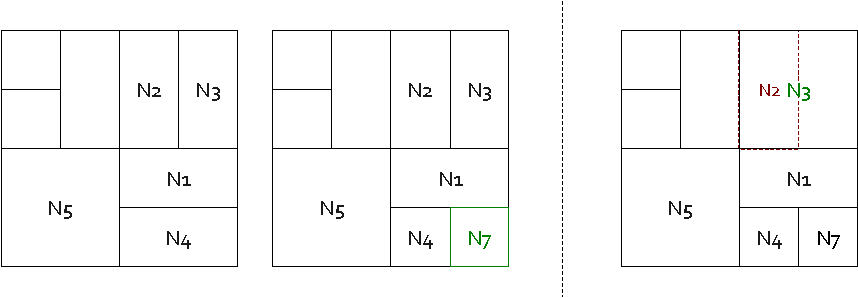
\includegraphics{grafics/can_new_node.pdf}
\caption{Eintritt und Fehlerfall bei CAN}
\label{fig:can_new_node}
\end{figure}

\Fref{fig:can_new_node} zeigt den Eintritt für Knoten N7. Nach Teilung der Zone von N4 verändert sich die Nachbarschaft von N1: Knoten N7 kommt neu hinzu. Die Nachbarschaft von $N1$ ist dann $\{N2, N3, N4, N5, N7\}$. Auf der rechten Seite ist der Ausfall des Knotens $N2$ (rot) dargestellt. Knoten $N3$ ist nun für die vereinigte Zone zuständig.

Ausstehende \texttt{UPDATE}-Nachrichten oder Timeouts weisen auf ausgefallene Knoten hin. Werden diese zum Routen einer Nachricht benutzt, stellt dies keine direkte Beeinträchtigung des Netzes dar, da die Nachricht über einen anderen Nachbarn verschickt werden kann. So könnte N1 auch N2 zum Nachrichtenversand nutzen, wenn N5 ausgefallen wäre (vergleiche \Fref[plain]{fig:can_routing}).

Ein Knoten, der einen ausfallenden Peer entdeckt hat, startet einen Timer, dessen Dauer proportional zur Zonengröße ist. Nach Ablauf sendet der Knoten eine spezielle \texttt{TAKEOVER}-Nachricht an alle Nachbarn des ausgefallenen Knotens\footnote{Dieses Wissen ist durch vorherige \texttt{UPDATE}-Nachrichten bekannt.}. Erreicht eine \texttt{TAKEOVER}-Nachricht einen Knoten, der den Ausfall ebenfalls bemerkt hat, stoppt dieser seinen eigenen Timer, falls seine Zone größer als die des Senders ist. Andernfalls antwortet er selbst mit seiner \texttt{TAKEOVER}-Nachricht. Auf diese Weise wird der Nachbar mit der kleinsten Zone gefunden. Dieser ist nun der neue Besitzer der Zone und fügt seine beiden Zonen zusammen, wie es in \Fref{fig:can_new_node} am Beispiel von N2 und N3 ersichtlich ist. N2 (rot dargestellt) ist ausgefallen und N3 vergrößert seine Zone. N2 ist nun nicht mehr in der Nachbarschaft von N1 enthalten. Es ist möglich, dass ein Knoten Besitzer zweier Zonen wird, welche sich nicht als eine Zone darstellen lassen. Ein Beispiel hierfür ist Knoten N4, der beim Ausfall von N5 dessen Zone übernimmt. Ein Hintergrundprozess defragmentiert solche Zonen und weist Knoten gegebenenfalls neue Koordinaten zu. Eine periodische Auffrischung der Datensätze soll auch hier einen Verlust im Fehlerfall schnell kompensieren.

Möchte ein Knoten $l$ das System verlassen, so sucht er einen Nachbarn mit der kleinsten Zone und sendet diesem seine Daten. Dieser Nachbar informiert nun die alten Nachbarn von $l$ über die geänderte Nachbarschaft.


\section{Auswahl des p2p-Netzwerkes}
Nach der Vorstellung der verschiedenen Netzwerke werden diese im Folgenen verglichen um ein geeignetes System als Netzwerk für \ac{m2etis} zu finden. Jedes System hat eigene Schwächen und Stärken. So bezahlt CAN einen günstigen Ein- und Austritt der Knoten dank der kleinen Nachbarschaft mit mehr Routing Hops als beispielsweise Chord. Dieses hat durch seine Fingertabelle wiederum mehr Einfluss auf das Routing, aktualisiert diese Tabellen jedoch erst nachträglich im Hintergrund während dies bei Pastry aktiv geschieht.

\Fref{tab:evaluation_fazit} (Auszug aus \cite{Goetz2005}) listet die durchschnittlich anfallenden Kosten (Routing Hops, Größe der Routinginformation, Nachrichtenanzahl beim Ein- und Austritt) für die drei getesteten System auf. $n$ ist die Anzahl der Knoten, $b$ die Anzahl der Bits der darstellenden Basis bei Pastry und $d$ die Anzahl der Dimensionen bei CAN.

\begin{table}[htbp]
\centering
\begin{tabular}{lcccc}
\toprule
 & Routing Hops & Routinginformation & Eintritt & Austritt\\ 
 \cmidrule{2-5}
Chord & $O(\frac{1}{2}log_2~n)$ & $O(2log_2~n) $ & $ O(log_2^2 n) $ & $ O(log_2^2 n) $ \\
Pastry & $O(\frac{1}{b}log_2~n)$ & $O(\frac{1}{b} (2^b-1) log_2~n) $ & $ O(log_{2^b}~n) $ & $ O(mlog_b~n) $ \\
CAN & $O(\frac{d}{2}n^\frac{1}{d})	$ & $O(2 d) $ & $ O(\frac{d}{2}n^\frac{1}{d}) $ & $ O(2 d) $ \\
\bottomrule
\end{tabular}
\caption[Vergleich der Systeme Chord, Pastry und CAN]{Vergleich der Systeme Chord, Pastry und CAN anhand einiger Gesichtspunkte}
\label{tab:evaluation_fazit}
\end{table}

Für uniformes Routing (d.h. das Routing ist bei allen Peers gleich) sind $O(log~n)$ beziehungsweise $O(n\frac{1}{d})$ Hops für Routingtabellen der Größe $O(log~n)$ beziehungsweise $O(d)$ die asymptotischen Grenze \cite{Xu2004Fundamental}. Die vorgestellten \ac{dht}-basierten Netzwerke nutzen ein uniformes Routing.


\paragraph{Geringe Latenz und Kommunikation über das Netzwerk}
Bei Pastry/Tapestry sind die kürzesten Routen und damit auch oftmals geringste Latenz im Nachrichtenversand zu erwarten, da die Routingtabelle im Vergleich zu Chord und CAN mehr Einträge enthält und diese einfacher mit - aus Netzwerksicht - nahen Peers belegt werden kann. Bei CAN hingegen wird das langsamste Routing erwartet, da Nachrichten nur zwischen benachbarten Knoten ausgetauscht werden. Sprünge (via Fingertabellen) sind nicht vorgesehen. Die Erwartungen decken sich mit den Werten in \Fref{tab:evaluation_fazit}.

Li stellt für verschiedene Parametereinstellungen der Netzwerke deren Bandbreite und Latenz gegenüber und untersucht dabei das Verhalten bei gehäuften Ein- und Austritten von Knoten. Hier ist Chord leicht im Vorteil, da lediglich der Verweis auf den Nachfolgeknoten für das korrekte Routing erforderlich ist. Bei allen Netzwerken pendelt sich die Latenz im \emph{worst case} auf 250ms ein \cite{Li2004Comparing}.

Die Vorteile der Kommunikation bei Pastry/Tapestry überwiegen für unseren Anwendungsfall.

\paragraph{Skalierbarkeit}
CAN steht hier an erster Stelle, da Ein- und Austritte von Peers nur wenige Knoten im Netz betreffen. Auch bei vielen Ein- und Austritten leidet das Netz unter keiner großen Nachrichtenlast. Allerdings leidet die Kommunikation in großen Netzen (siehe obigen Punkt). Chord liegt auf dem letzten Platz, da das Netzwerk erst durch später aufgerufene Methoden vollkommen funktionsfähig wird (siehe \emph{Eintritt und Austritt (Fehlerfall) von Knoten}).  Pastry und Tapestry liegen auf Zweitem Platz; der Aufbau der Routingtabelle erfolgt in vielen kleinen Schritten - dafür ist ein Knoten danach ein vollwertiger Peer im System.

\paragraph{Fehlertoleranz bei Knotenausfall}
Alle Systeme finden ausgefallene Knoten durch periodisch versandte Nachrichten an benachbarte Peers oder durch Timeouts verschickter Nachrichten. Jedes System kompensiert solch einen Fall auf eigene Art und Weise. Bei CAN wird ein Knoten seine mit der verlassenen Zone verbinden, Knoten in Chord aktualisieren ihre Fingertabellen und Peers in Pastry und Tapestry versuchen durch Befragungen anderer Knoten die entstandene Lücke in der Routingtabelle zu füllen. Ein Knotenausfall hat bei CAN allerdings die geringsten Auswirkungen auf das restliche System, da nur die Nachbarknoten involviert sind. Dies ist der kleinen Routingtabelle geschuldet.

Alle Systeme fordern jedoch die Applikation zu einer periodischen Auffrischung der gespeicherten Daten auf und bieten selbst kaum Redundanz (Ausnahme Tapestry) an.


\paragraph{Bestimmung der Nachbarschaft}
Allein die Größe der Routingtabelle bedingt, dass bei Pastry und Tapestry mehr Einfluss auf die Zusammenstellung genommen werden kann. Bei CAN gibt es faktisch nur eine Entscheidung bei Eintritt in das Netz, Chord bietet über die Fingertabelle minimalen Einfluss, während bei Pastry explizit das Neighborhood Set eingesetzt wird, um eventuelle Lücken in der Routingtabelle geschickt zu besetzen.

\paragraph{Eingriff in Routingentscheidungen}
Das Routing bei CAN kann nur bedingt beeinflusst werden. Chord hingegen bietet mit seiner Fingertabelle mehr Variationsmöglichkeiten - allerdings nur für die zu überbrückende Distanz im Schlüsselraum. Pastry und Tapestry verbinden diese Variationen mit vielfältigen Nachbarschaftsoptionen.

Zusammenfassend zeigen die obigen Punkte, dass Pastry/Tapestry als Netzwerk für \ac{m2etis} gut geeignet ist. Pastry selbst ist als Javabibliothek\footnote{\url{http://www.freepastry.org}} verfügbar und die Entwicklung von Tapestry (ebenfalls in Java implementiert) wurde mit Version 2.01 eingestellt. Chimera \cite{Allen2006Chimera} ist der Nachfolger von Tapestry und vereint das Beste von Pastry und Tapestry in sich\footnote{siehe \url{http://current.cs.ucsb.edu/projects/chimera/index.html}}: 
\begin{quote}
Chimera is a light-weight C implementation of a ``next-generation'' structured overlay that provides similar functionality as prefix-routing protocols Tapestry and Pastry.  Chimera gains simplicity and robustness from its use of Pastry's leafsets, and efficient routing from Tapestry's locality algorithms.  In addition to these properties, Chimera also provides efficient detection of node and network failures, and reroutes messages around them to maintain connectivity and throughput.  
\end{quote}

Der frei verfügbare Code (veröffentlicht unter GPL), die Anpassbarkeit und die Unterstützung der Zielplattformen Linux und Windows sprechen für Chimera. Weiterhin entspricht Chimera der generischen \ac{api} und kann bei gravierenden Problemen durch ein anderes System ausgetauscht werden, ohne das restliche System zu beeinflussen. Die Konzeption des Netzwerkes ist ausschlaggebender als eigentliche Implementierung und daher wird Chimera als Netzwerk für \ac{m2etis} gewählt.

In diesem Kapitel wurden die drei Netzwerke Chord, Pastry/Tapestry und CAN verglichen und ihre unterschiedlichen Arbeitsweisen erklärt. Es zeigt sich, dass das Konzept von Pastry/Trapestry für \ac{m2etis} gut geeignet ist. Damit ist der erste Teil dieser Arbeit, die Auswahl eines geeigneten Netzwerkes, abgeschlossen. Das nächste Kapitel befasst sich nun mit der Konzeption der Publish/Subscribe-Komponente, die auf diesem Netzwerk aufsetzt.
